\documentclass[11pt, oneside]{article}
\usepackage[margin=1in]{geometry}
\geometry{letterpaper}
\usepackage{booktabs}
\usepackage{hyperref}
\usepackage{enumitem}
\usepackage{float}
\usepackage{caption}
\usepackage{subcaption}
\usepackage[numbers]{natbib}
\usepackage{graphicx}
\usepackage{amssymb}
\usepackage{amsmath}
\usepackage{array}
\usepackage{longtable}
\usepackage{xcolor}
\usepackage{tabularx}
\usepackage{setspace}
\usepackage{tikz}
\usetikzlibrary{positioning,arrows.meta}

\hypersetup{
    colorlinks=true,
    linkcolor=blue,
    citecolor=blue,
    urlcolor=blue
}
\graphicspath{{figures/}}
\captionsetup{font=small,skip=4pt}
\setlength{\textfloatsep}{8pt}
\setlength{\floatsep}{6pt}
\setlength{\intextsep}{6pt}
\newcommand{\A}{\textsf{A}}\newcommand{\B}{\textsf{B}}\newcommand{\C}{\textsf{C}}\newcommand{\D}{\textsf{D}}

% ============================================================
% TITLE BLOCK --- students must keep this format
% Filename of the compiled PDF must be:
% CS781-CP-[Firstname]-[Lastname]-[RollNo]-report.pdf
% ============================================================
\title{CS781 Capstone Project:\\
In-House Legal Intelligence System}
\author{
    Rohit Batra  \\
    261110054 \\
    {\tt \textcolor{red}{[userid]}@iitk.ac.in}\\
    Indian Institute of Technology Kanpur (IIT Kanpur)
}
\date{}

\begin{document}
\maketitle

\begin{abstract}
A law firm that cannot send client documents to external services needs legal NLP it can host itself. We built a seven-phase pipeline under that constraint. Phase~1 pretrains four compact language models from scratch on the official corpus (103--139M parameters: decoder-only Transformer, encoder--decoder, LSTM and dilated TCN) with our own 50K BPE tokenizer and an equal source mix. Every later model starts from these weights and adapts them, with LORMA, LoRA, IA$^3$, prefix and prompt tuning, adapters, layer-wise fine-tuning and knowledge distillation, to entity recognition, rhetorical roles, judgment prediction, statute identification, summarisation and prior-case retrieval. The decoder transferred best to five of six tasks. Reading the right part of long documents, a probe-then-fine-tune schedule that ended repeated training collapses, and per-label calibration moved the scores most. Distilled students two-thirds the size kept their teachers' quality, twice exceeding it.
\end{abstract}

% ============================================================
\section{Competition Result}
% ============================================================
\noindent
\textbf{Codabench username:} \texttt{r\_261110054}
\hfill
\textbf{Roll number:} 261110054

\begin{table}[H]
\centering\small
\caption{Official phase scores and ranks (best valid submission per phase). Ranks recorded on 4 November 2026.}
\label{tab:leaderboard}
\begin{tabular}{clccc}
\toprule
Phase & Task & Primary metric (value) & Rank & Valid submissions \\
\midrule
1 & Legal LM Pretraining & BERTScore F1 (0.8058) & 133 & 4 \\
2 & Legal NER & Strict Macro-F1 (0.4912) & 83 & 4 \\
3 & Rhetorical role prediction & Macro-F1 (0.5184) & 47 & 7 \\
4 & Court judgment prediction & Macro-F1 (0.6795) & 91 & 7 \\
5 & Legal statute identification & Macro-F1 (0.3037) & 107 & 4 \\
6 & Abstractive summarization & BERTScore F1 (0.8354) & 77 & 8 \\
7 & Prior case retrieval & Micro-F1@7 (0.2534) & 0$^{*}$ & 4 \\
\bottomrule
\end{tabular}

\smallskip{\footnotesize $^{*}$The Phase-7 leaderboard was still changing when ranks were recorded, so no rank is given.}
\end{table}

\noindent
\textbf{Total valid Codabench submissions across all phases:} 38
\quad
\textbf{Date ranks were recorded:} 4 November 2026

\medskip
We met the minimum of four distinct submissions in every phase; each covers all four Phase-1 backbones (Phase~7: three backbones and a distilled student). Extra runs in Phases 3, 4 and 6 were improved or decoding-only re-runs, so four or five distinct experiments are counted per phase (full list: \texttt{results/submissions.csv} in \href{https://github.com/Rohit2004Batra/cs781-legal-lm-capstone}{the repository}).

% ============================================================
\section{Introduction and Problem Description}
% ============================================================
Client confidentiality rules out sending judgments to a hosted language model, so a firm needs models it trains and runs itself, built here from only the official \texttt{Exploration-Lab/CS-781-Capstone} data. Phase~1 pretrains a language model of 50M--300M parameters from scratch; its test is to continue 1,000 legal prompts of 512 words with 128 words, scored by BERTScore F1~\cite{zhang2020bertscore}, ROUGE-L~\cite{lin2004rouge} and BLEU~\cite{papineni2002bleu}. Phases 2--7 adapt that model to six tasks: character-level NER over 12 entity types (strict Macro-F1, so a span one character off is wrong); one of 13 rhetorical roles per sentence in Corporate Law and IT judgments (Macro-F1); binary judgment prediction (Macro-F1); multi-label identification of 100 statutes (Macro-F1 over statutes); headnote-style summarisation (BERTScore F1); and prior-case retrieval returning exactly seven candidates per query (Micro-F1@7). Every experiment starts from our own Phase-1 weights (no other pretrained model, external corpus or LLM API); each phase needs four distinct submissions including LORMA~\cite{bihany2025lorma} and knowledge distillation; compute was free Kaggle T4 GPUs.

We asked whether different architectures transfer differently, which adaptation suits which backbone, how to represent very long documents, how much calibration matters, and whether distilled students keep their teachers' quality. Phases were not pipelined into one another, so each is a clean test of transfer from Phase~1.

% ============================================================
\section{Data Analysis and Preprocessing}
% ============================================================
\subsection{Sources and official splits}
We used only the official phase folders, downloaded inside each notebook. Table~\ref{tab:data} gives sizes and the analysis finding that changed each design. Phases 2 and 6 have no official dev set, so we held out 14 of 70 and 150 of 7,030 documents.

\begin{table}[t]
\centering\footnotesize\setlength{\tabcolsep}{4pt}
\caption{Data per phase and the analysis result that shaped the design.}\label{tab:data}
\begin{tabularx}{\textwidth}{@{}c p{3.6cm} X@{}}\toprule
Ph. & Train / dev / test & Finding $\rightarrow$ decision \\\midrule
1 & 4.34B tokens; 2\% held out & High courts and tribunals are 91\% of tokens (acts 3.5\%) $\rightarrow$ sample the four sources equally. \\
2 & 70 (2 folds) / -- / 35 docs; 8,393 spans & Only 3.8\% of gold starts lie on a BPE token start (the leading space is part of the token) $\rightarrow$ predict boundaries per character. \\
3 & 80 / 10 / 10 docs; 17k sentences & Median sentence 32 tokens, documents up to 70k; Issue is 0.2\% of CL $\rightarrow$ sentence encoder + document BiLSTM, class weights. \\
4 & 31.6k unique / 3,505 / 1,517 & \textbf{All test cases also occur in dev, with labels} $\rightarrow$ never train or tune on them (``dev-clean'', 1,988 cases). Outcome words differ only near the end $\rightarrow$ read the last chunks. \\
5 & 42.8k / 10.2k / 13.0k; 100 IDs & 3.7 statutes per case; 42\% of dev label sets unseen in train $\rightarrow$ independent sigmoids, per-statute thresholds. \\
6 & 7,030 / -- / 100 & Summaries are 22\% of document length, drawn from the whole case; 4\% novel words $\rightarrow$ summarise every chunk and join. \\
7 & 827 / 118 / 237 queries & Each query is in its own pool; median 4--5 relevant; BM25 scores 0.13 on full text, 0.33 on the first 2,000 words $\rightarrow$ exclude the query; use first and last chunks. \\\bottomrule
\end{tabularx}
\end{table}

\subsection{Corpus statistics that informed design}
A uniform Phase-1 sample would be dominated by High Court style, so each training window draws a source with equal probability (acts upsampled about $7\times$). NER labels are skewed (DATE 1,575 spans, R.COUNSEL 184; median span 13 characters, maximum 233). Rhetorical roles follow a document order (facts, arguments, precedents, ratio, ruling), and CL dev has far more argument sentences than IT (41\% vs 12\%). In Phase~4, train is 59/41 while dev and test are balanced; ``set aside'' appears in the last 1,000 characters of 25\% of label-1 and 6.6\% of label-0 cases, with equal rates in the first 1,000. Statute frequencies span $43\times$ (272 to 11,730 cases) and pairs co-occur strongly ($P(28\mid20)=0.93$). In Phase~7 the oracle ceiling with exactly seven answers is only 0.62, because 13\% of dev queries have one relevant case and a third have more than seven.

\subsection{Preprocessing decisions}
Text was kept cased (38K of 50K tokens contain capitals), except in Phase~4, whose dev and test splits are lower-case. Masked placeholders (3--5 BPE tokens each) became one plain word (\texttt{<SECTION>}$\rightarrow$``Section'') or were removed where they also hide ordinary words (\texttt{<ENTITY>}).

Phase-2 whitespace was never normalised: each 512-token window keeps a character-to-token map from the tokenizer's offsets, and decoding the gold boundaries through this path reproduces all 1,861 validation spans exactly. Phase~3 used the provided sentence lists unchanged; Phases 4--7 split cases into 510-token chunks (sentence-aligned 1,200-token chunks in Phase~6) and select chunks per task (Section~\ref{sec:approach}).

% ============================================================
\section{Approach and Model Evolution}\label{sec:approach}
% ============================================================
\subsection{Phase-1 foundation model}
We trained our own byte-level BPE tokenizer (vocabulary 50,000; 25M characters per source; \texttt{[PAD] [UNK] [BOS] [EOS]}), so legal tokens such as ``Section'' and ``appellant'' get their own entries.

The four architectures are \A{}, a pre-LayerNorm decoder-only Transformer~\cite{vaswani2017attention} (12 layers, $d$=768, 12 heads, GELU FFN 3,072, learned positions, context 2,048, tied embeddings; 125.0M); \B{}, a 6+6-layer encoder--decoder with shared embeddings that predicts the next 1,024 tokens from the previous 1,024 (139.3M); \C{}, a three-layer LSTM~\cite{hochreiter1997lstm} with 1,280 units (103.4M); and \D{}, a TCN~\cite{bai2018tcn} of 10 residual blocks of weight-normalised causal convolutions with dilations 1--512 and a 4,093-token receptive field (114.2M).

We chose four families on purpose, each with a different inductive bias under the same budget. The decoder matches the Phase-1 task (continue the text) and attends over its whole 2,048-token context. The encoder--decoder reads the prompt bidirectionally before generating, and its encoder is a natural feature extractor for the classification phases. The stacked LSTM runs in linear time with constant memory over documents of any length, and its step-by-step state suits local decisions such as entity boundaries. The TCN is fully parallel but has a fixed, very wide receptive field with no attention cost. Comparing attention, recurrence and convolution shows which bias transfers best to each task.

Each notebook asserts its parameter count lies within 50M--300M. All four were trained with next-token cross-entropy on 100M tokens (2.3\% of the corpus, the most Kaggle sessions allowed). We used AdamW ($\beta=(0.9,0.95)$, weight decay 0.1), a learning rate of $3\times10^{-4}$ with cosine decay to $3\times10^{-5}$, 16K tokens per step and bf16, and selected checkpoints on the held-out loss.

Decoding produced exactly 128 words, near-greedy for \A{} and \C{} (temperature 0.1, top-$p$ 0.95), temperature 0.7 with repetition penalty 1.1 for \B{}, and temperature 0.8 for \D{}. Untuned near-greedy decoding made \A{} repetitive: lowest perplexity (20.3 vs 31.8, 48.0, 48.2) but lowest BERTScore (0.793 vs 0.806, 0.802, 0.805).

\subsection{Transfer protocol (Phases 2--6, and 7)}
Every downstream model starts from a Phase-1 checkpoint plus a task head (Figure~\ref{fig:system}).

We implemented full and layer-wise fine-tuning, BitFit~\cite{benzaken2022bitfit}, LoRA~\cite{hu2022lora}, IA$^3$~\cite{liu2022ia3}, prefix~\cite{li2021prefix} and prompt tuning~\cite{lester2021prompt}, Houlsby and bottleneck adapters~\cite{houlsby2019adapters}, knowledge distillation (KD)~\cite{hinton2015distilling}, and LORMA~\cite{bihany2025lorma}, a multiplicative update $W_{\text{eff}}=(I+\tfrac{\alpha}{r}BA)\,W_0$ with $r$=8, $\alpha$=16 and $B$=0 at the start, applied to q/k/v/out/fc1/fc2 of \A{} and to the recurrent gate matrices of \C{}.

Two pieces of infrastructure carry across phases. First, \A's residual stream has a few nearly constant dimensions ($|x|\approx46$ against a mean of 2), so chunk features are \emph{standardised per dimension}. Second, from Phase~4 on we used \emph{LP-FT}~\cite{kumar2022lpft}: a probe (or retrieval projection) fit on cached frozen features becomes ``epoch~0'', adapter and head are then fine-tuned at $10^{-4}$, and the best epoch on validation is kept.

\begin{figure}[t]\centering\small
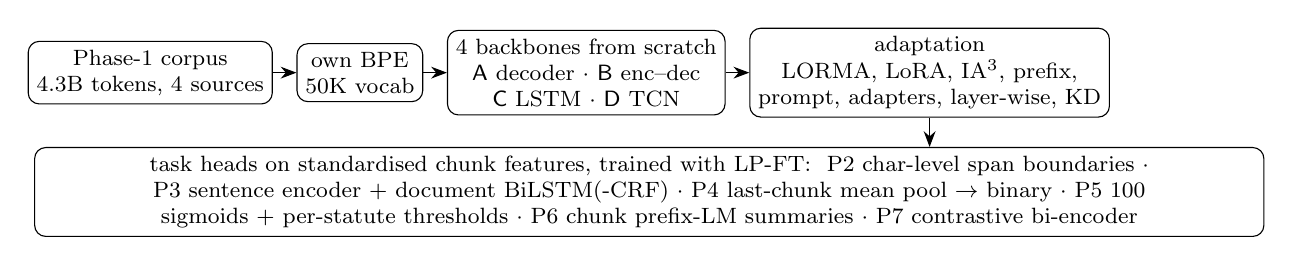
\begin{tikzpicture}[node distance=3mm and 3mm, box/.style={draw,rounded corners,align=center,inner sep=3pt,font=\footnotesize}, >={Stealth[length=2mm]}]
\node[box] (corpus) {Phase-1 corpus\\4.3B tokens, 4 sources};
\node[box,right=of corpus] (tok) {own BPE\\50K vocab};
\node[box,right=of tok] (bb) {4 backbones from scratch\\\A{} decoder $\cdot$ \B{} enc--dec\\\C{} LSTM $\cdot$ \D{} TCN};
\node[box,right=of bb] (peft) {adaptation\\LORMA, LoRA, IA$^3$, prefix,\\prompt, adapters, layer-wise, KD};
\node[box,below=4mm of bb,xshift=8mm,text width=15.4cm] (heads) {task heads on standardised chunk features, trained with LP-FT: \ P2 char-level span boundaries $\cdot$ P3 sentence encoder + document BiLSTM(-CRF) $\cdot$ P4 last-chunk mean pool $\rightarrow$ binary $\cdot$ P5 100 sigmoids + per-statute thresholds $\cdot$ P6 chunk prefix-LM summaries $\cdot$ P7 contrastive bi-encoder};
\draw[->] (corpus)--(tok); \draw[->] (tok)--(bb); \draw[->] (bb)--(peft); \draw[->] (peft.south)--(peft.south|-heads.north);
\end{tikzpicture}
\caption{System overview: one set of Phase-1 backbones, separately adapted copies for each phase.}\label{fig:system}
\end{figure}

\subsection{Phase 2 --- Legal NER}
Since almost no gold start lies on a token start, we built a character-level span head: each character receives its token's backbone state plus a 32-dimensional character embedding, a small convolution follows, and two heads give start and end probabilities for each label. Training uses binary cross-entropy with a positive weight capped at 30 (boundaries are 0.01--0.08\% of characters) and output biases initialised from label prevalence; 512-token windows overlap with stride 384 and are averaged in character space. Decoding pairs each start above its label's threshold with the best end within a per-label length cap (both tuned on validation) and resolves overlaps. The best system, \C{} with LORMA on the recurrent weights, trains 0.79M parameters; an earlier additive adapter (not true LORMA) scored 0.372 against 0.392 before calibration.

\subsection{Phase 3 --- Rhetorical role prediction}
Each sentence ($\leq$128 tokens) is encoded into [mean; final state], projected to 512 dimensions with a domain embedding and relative position; a two-layer document BiLSTM over 128-sentence windows adds context, and from S7 on a linear-chain CRF~\cite{lafferty2001crf} decodes roles with Viterbi. CL and IT are trained jointly (40 documents each is too few) with class weights $(N/Kn_c)^{0.5}$ capped at 10.

The best submission (S6) is a KD student keeping layers 0, 2, \ldots, 10 of \A{} (DistilBERT-style~\cite{sanh2019distilbert}) with LoRA, trained with CRF NLL, weighted cross-entropy and $T^2\cdot\mathrm{KL}$ ($T=2$) against the S7 teacher, then retrained on train+dev for the epoch count chosen on dev.

\subsection{Phase 4 --- Court judgment prediction}
Each case is represented by its last two chunks of 510 tokens. A chunk vector [mean; final state] is standardised, the chunk vectors are averaged, and a linear layer gives the two-class output. Train is 59/41 while test is balanced, and a majority-class predictor scores $\approx$0.33 Macro-F1 (what our collapsed runs produced); class-weighted cross-entropy and a threshold tuned on dev-clean (0.41) handle the shift.

\subsection{Phase 5 --- Legal statute identification}
Up to 8 chunks are selected: the first, the last, and those with the most ``Section'' or ``Act'' tokens. Each case is pooled as [mean; max] over chunks and passed to 100 independent sigmoids, trained with binary cross-entropy whose positive weight is $\sqrt{\text{neg}/\text{pos}}$, capped at 10. Every statute has at least 68 dev positives, so each gets its own threshold; we report cross-fitted estimates (tuned on half of dev, scored on the other half) and give every case at least one statute. Rare statutes are handled by the capped positive weight and per-statute thresholds rather than resampling.

\subsection{Phase 6 --- Abstractive summarisation}
Only 19\% of documents fit in 2,048 tokens, so we use sentence-aligned 1,200-token chunks. Each summary sentence is assigned to the chunk that contains its best-matching source sentence (89\% match with word recall $\geq0.5$). \A{} with LORMA is trained as a prefix language model on \texttt{[BOS] chunk ``Summary:'' target [EOS]}. At inference every chunk is summarised with a KV cache and 4-gram blocking, and the chunk summaries are joined with duplicate sentences removed.

The original decoding was short and repetitive (20--39\% repeated trigrams); a grid on 60 validation documents chose a minimum length of 22\% of each chunk and a CTRL repetition penalty~\cite{keskar2019ctrl} of 1.2. The tuned runs replaced the originals.

\subsection{Phase 7 --- Prior case retrieval}
We built a bi-encoder in the style of dense retrieval~\cite{karpukhin2020dpr}. Each chunk's [mean; final state] features are standardised and projected to 256 dimensions; the case vector is the normalised mean over the first 8 and last 8 chunks, and candidates are ranked by cosine similarity with the query removed from its own ranking. Training uses InfoNCE~\cite{oord2018infonce} at temperature 0.05 over one relevant case, two hard negatives from the TF-IDF top 50 and all in-batch documents. BM25~\cite{robertson2009bm25} and TF-IDF only served as references and negative miners. The KD student (S4) keeps 6 of \A's 12 layers and matches the teacher's in-batch similarity distribution ($T^2\cdot\mathrm{KL}$, $T=2$), plus one teacher-mined hard negative per pair.

\subsection{Final submitted system}
The submitted systems are \B{} in Phase~1, \C{}+LORMA S3 with the calibrated decoder in Phase~2, the S6 student (stage~2) in Phase~3, and \A{}+LORMA S1 in Phases 4--7 (Phase~6 with tuned decoding); Table~\ref{tab:hparams} gives their settings, and each checkpoint is a Kaggle dataset linked from the phase README.

% ============================================================
\section{Experiments and Implementation Details}
% ============================================================
\subsection{Compute and training protocol}
All 46 training notebooks ran on Kaggle T4s (two with DataParallel after Phase~1), 30--160 minutes each. Notebooks save \texttt{latest.pt} (with optimiser, scheduler and sampler state) every few hundred steps, so a run interrupted by a session limit resumes exactly.

Downstream runs used AdamW (weight decay 0.01), linear warm-up over 3--6\% of steps then linear decay, clipping at 1.0 and fp16; checkpoints were selected on the validation task metric (validation loss in Phase~6).

\begin{table}[t]
\centering\scriptsize\setlength{\tabcolsep}{1.8pt}
\caption{Hyperparameters of the final model in each phase (total parameters; trainable in brackets).}
\label{tab:hparams}
\begin{tabular}{lccccccc}
\toprule
 & P1 \B & P2 \C+LORMA & P3 KD student & P4 \A+LORMA & P5 \A+LORMA & P6 \A+LORMA & P7 \A+LORMA \\
\midrule
Params (M) & 139.3 & 104.2 (0.79) & 85.5 (3.04) & 126.4 (1.4) & 126.7 (1.63) & 126.4 (1.33) & 126.7 (1.72) \\
Context & 1k$\rightarrow$1k & 512/384 & 128/sent. & 2$\times$510 & $\leq$8$\times$510 & 1,200+640 & 16$\times$510 \\
Peak LR & 3e-4 & 2e-4 & 3e-4/1e-3 & 1e-4 & 1e-4 & 2e-4 & 1e-4 \\
Batch$\times$acc & 1$\times$8 & 2$\times$1 & 128 sent. & 8 cases & 16 ch.$\times$2 & 4$\times$4 & 4 pairs \\
Epochs & 6,104 steps & 3 (best 2) & 20 (best 17) & 4 (best 3) & 3 & 2 & 3 (best 2) \\
Dropout & 0.1 & 0 (frozen) & 0.2 head & 0 & 0.1 head & 0 & 0 \\
Decode/thr. & $T$0.7, rep 1.1 & thr.+caps & Viterbi & thr.\ 0.41 & per-statute & 22\%, rep 1.2 & top-7 cosine \\
\bottomrule
\end{tabular}
\end{table}

\subsection{Local evaluation}
Every phase has a labelled held-out set that never touches test labels: 2\% of documents held out by hash (P1), 14 of 70 labelled documents (P2), the official dev sets (P3, P5, P7), dev minus the 1,517 test cases (P4), and 150 training documents (P6). Each notebook implements the official metric and validates \texttt{prediction.json} (all and only test IDs, exact types, per-phase constraints such as seven unique pool IDs excluding the query).

Our first Phase-3 score used a Macro-F1 over present labels only (0.476 vs Codabench's 0.402), so we switched to the 13-label average. Local and test scores agree closely (plot in \texttt{results/plots}): the cross-fitted Phase-5 estimates were within $\pm0.01$ of test for all four runs. The largest gaps came from the smallest sets (10 documents in Phase~3; 118 queries in Phase~7, where every run lost 0.02--0.04).

\subsection{Ablations and controlled comparisons}
Table~\ref{tab:abl} changes one factor at a time. Document structure and decision calibration produced the largest effects, larger than switching adapters on a fixed backbone; prefix tuning lost to LoRA under an identical pipeline, and max pooling lost badly to mean pooling for retrieval.

\begin{table}[t]
\centering\footnotesize\setlength{\tabcolsep}{4pt}
\caption{Controlled ablations on validation (Phase~6 in ROUGE-1).}\label{tab:abl}
\begin{tabular}{clr|clr}\toprule
Ph. & Change (all else fixed) & $\Delta$ & Ph. & Change (all else fixed) & $\Delta$ \\\midrule
2 & per-label span caps + thresholds & +0.102 & 5 & first chunk only vs evidence chunks & $-$0.035 \\
3 & document BiLSTM vs sentence-only & +0.158 & 5 & thresholds scored on tuning data & +0.015 bias \\
3 & Viterbi CRF vs argmax & +0.042 & 6 & all chunks joined vs first chunk & +0.158 \\
3 & prefix tuning vs LoRA (test) & $-$0.049 & 6 & tuned decoding, same weights & +0.060 \\
4 & last 2 vs first 2 chunks & +0.102 & 7 & contrastive proj.\ on frozen \C & +0.074 \\
4 & LORMA fine-tuning over its probe & +0.088 & 7 & mean vs max pooling over chunks & +0.089 \\
4 & 4 epochs vs 2 (same recipe) & +0.024 & 7 & first 8+last 8 vs first chunk & +0.157 \\\bottomrule
\end{tabular}
\end{table}

% ============================================================
\section{Results}
% ============================================================
Table~\ref{tab:main} gives every counted submission. In Phase~1, \B{} had ROUGE-L 0.162 and BLEU-4 0.015 (best: \D{}, 0.185 and 0.021). Best-run secondary metrics: P4 precision/recall 0.662/0.744, P5 Micro-F1 0.399, P6 ROUGE-1/L 0.527/0.240, P7 P@7/R@7 0.259/0.248.

\begin{table}[t]
\centering\scriptsize\setlength{\tabcolsep}{3pt}
\caption{Counted submissions: local validation and official test scores, in the order listed (best per phase in bold; trainable parameters in \texttt{results/submissions.csv}).}\label{tab:main}
\begin{tabularx}{\textwidth}{@{}c X >{\raggedleft\arraybackslash}p{3.3cm} >{\raggedleft\arraybackslash}p{3.4cm}@{}}\toprule
Ph. & Submissions: backbone + technique & Local & \textbf{Test} \\\midrule
2 & S1 \A{} full FT / S2 \B{} enc.+LoRA / \textbf{S3 \C{}+LORMA} / S4 KD \D{}$\rightarrow$6-block \D{} & .225 / .198 / .494 / .220 & .192 / .177 / \textbf{.491} / .253 \\
3 & S1 \C{}+LORMA / S3 \B{}+IA$^3$ / S4 \D{}+prompt / S7 \A{}+LoRA+CRF / \textbf{S6 KD S7$\rightarrow$6-layer \A} & .40 / .219 / .329 / .450 / .458 & .402 / .236 / .339 / .502 / \textbf{.518} \\
4 & \textbf{S1 \A{}+LORMA LP-FT} / S2 \C{} layer-wise / S3 \B{} BitFit / S4 \D{} adapters / S5 KD S2$\rightarrow$2-layer \C & .695 / .562 / .531 / .578 / .613 & \textbf{.680} / .562 / .491 / .527 / .592 \\
5 & \textbf{S1 \A{}+LORMA} / S2 \C{} layer-wise / S3 \D{} adapters / S4 KD ensemble$\rightarrow$\B{}+LoRA & .298 / .273 / .271 / .215 & \textbf{.304} / .263 / .273 / .220 \\
6 & \textbf{S1 \A{}+LORMA} / S2 \B{}+LoRA / S3 \D{} Houlsby / S4 KD \A$\rightarrow$\C{} (tuned decoding) & R1 .521 (S1) & \textbf{.835} / .809 / .814 / .816 \\
7 & \textbf{S1 \A{}+LORMA} / S2 \C{} layer-wise / S3 \D{} prompt / S4 KD S1$\rightarrow$6-layer \A & .269 / .217 / .198 / .280 & \textbf{.253} / .180 / .181 / .237 \\\bottomrule
\end{tabularx}
\end{table}

\begin{figure}[t]\centering
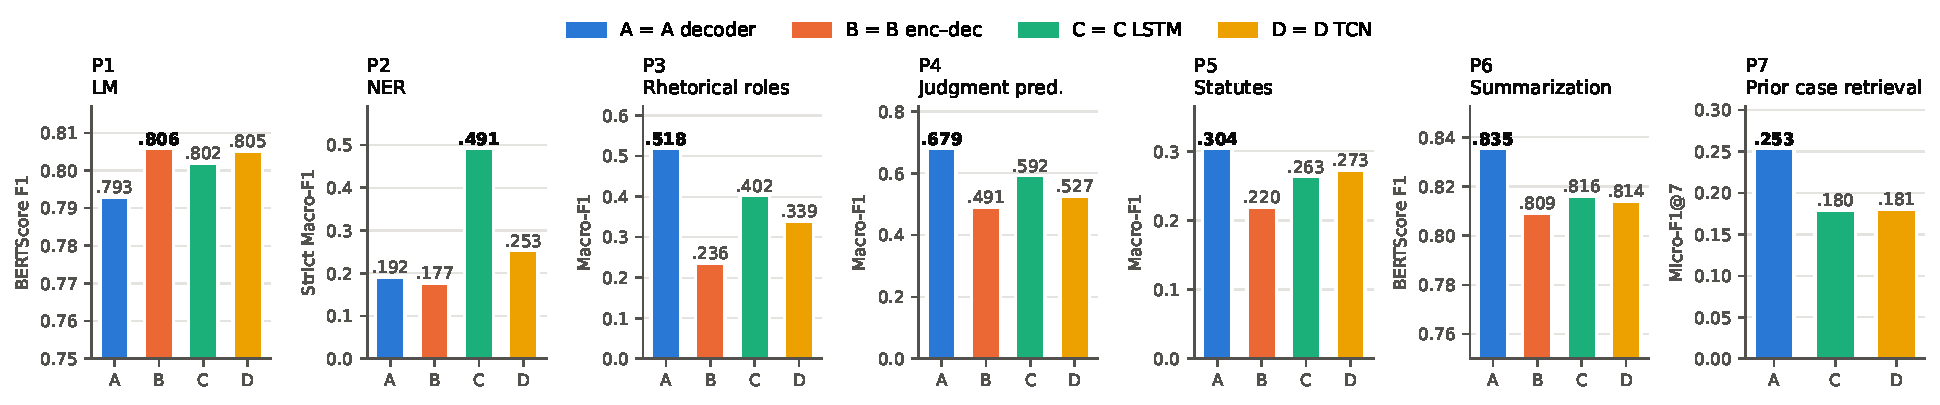
\includegraphics[width=\textwidth]{fig1_scores_by_phase_and_backbone.pdf}
\caption{Best official score per backbone and phase (KD students under their own backbone; Phase~6 with tuned decoding; no \B{} run in Phase~7; BERTScore axes start at 0.75). \A{} wins Phases 3--7; \C{} wins NER.}\label{fig:backbones}
\end{figure}

\textbf{Which system won, and why.} \A{} adapted with LORMA (or distilled from it) won five of six downstream phases (Figure~\ref{fig:backbones}), as frozen-feature probes predicted before any fine-tuning (Phase-3 sentence probes: \A{} 0.283, \C{} 0.235, \D{} 0.226, \B{} encoder 0.117; frozen Phase-7 retrieval: \A{} 0.238, \D{} 0.122, \C{} 0.112).

\A{} had seen the longest contexts and had the lowest perplexity, so its states encode more of the document, and LORMA reshapes every projection slightly while touching about 1\% of the parameters. NER is the exception: a boundary decision is local and character-precise, and the LSTM state, adjusted multiplicatively on the recurrent gates, gave the sharpest boundaries.

\textbf{Learning curves.} In LP-FT runs (Figure~\ref{fig:curves}) the probe (epoch~0) recovers most of the score; fine-tuning adds 0.02--0.09.

\begin{figure}[t]\centering
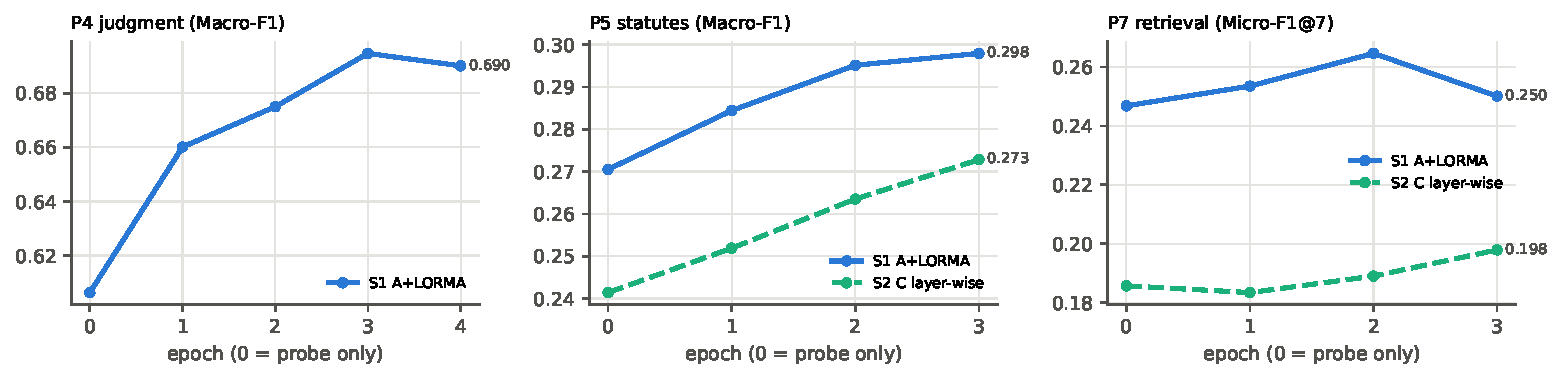
\includegraphics[width=0.72\textwidth]{fig5_lpft_curves.pdf}
\caption{Validation metric vs epoch for LP-FT runs; epoch 0 is the probe or projection alone.}\label{fig:curves}
\end{figure}

\textbf{Per-class results.} In NER (S3, validation) DATE (0.91), COURT (0.77) and STAT (0.73) are reliable; APP, AUTH, RESP, WIT and PREC (0.25--0.30) are weak. In rhetorical roles, Statute (0.80) and RulingByPresentCourt are easy, Issue and None stay weak, and ArgumentRespondent recall rose from 0.26 to 0.54 only with the CRF and KD. Per-statute F1 rises with frequency, from 0.20 (rarest quartile) to 0.45 (most frequent).


% ============================================================
\section{Error Analysis and Discussion}\label{sec:err}
% ============================================================
\subsection{Phase-wise failure modes}
\textbf{Phases 1--3.} Near-greedy \A{} fell into repetitive loops; all four models' continuations were legal in style but drifted from the prompt's topic, compressing BERTScore to a 0.013 range. In NER, the uncalibrated S3 model predicted spans up to 512 characters (gold spans are under 150) until per-label caps removed this; AUTH is over-predicted (436 false vs 105 true positives), and APP vs RESP hinges on a position relative to ``versus'' often far from the name. Role errors concentrate where the role depends on what the court later does with a sentence or on who is speaking, and on rare roles.

\textbf{Phase 4.} \A{} with LORMA collapsed to a constant prediction in four runs. Removing one suspected cause per run (attention pooling, outlier dimensions via standardisation, dropout in the frozen backbone) did not help: the cause was a randomly initialised head combined with multiplicative updates, which destroy the features before the head finds the weak signal. LP-FT fixed it (probe 0.606, fine-tuned 0.695). Remaining errors favour acceptance (recall 0.744, precision 0.662): with the ruling removed, partly allowed or remanded cases read like acceptances.

\textbf{Phase 5.} The dominant error swaps a specific statute for a frequent generic one (12--14 missed for 5; 34, 61, 77 missed for 97): with references masked, the model falls back on what is typical.

\textbf{Phases 6--7.} Chunk summaries are written independently, so facts are restated and the holding is sometimes split; longer tuned outputs raised ROUGE-1 and BERTScore but lowered ROUGE-L for three of four models. In retrieval, P@7 is 0.05--0.08 for single-answer queries, and recall 0.09--0.13 for queries with 16+ answers. S1 finds nothing for 18 of 118 dev queries. All four rankers stay below TF-IDF (0.368 on dev), but their hits differ: S1 and TF-IDF together find 393 relevant cases, against 331 for TF-IDF alone.

\subsection{What the metrics miss, limitations and next steps}
BERTScore and ROUGE reward similarity to one reference, so a fluent summary that misstates the holding can still score well. Strict span-F1 gives no credit for an entity one character off, and Micro-F1@7 caps any system at 0.62 on dev. The scores rank systems; they do not certify them.
Each Phase-1 model saw 2.3\% of the corpus and three were still improving; fine-tuning was held to 2--4 epochs; there was no human legal evaluation.

Next we would pretrain \A{} on 1B tokens with a 4,096 context, add contrastive pretraining on citing--cited training pairs, raise in-batch negatives with gradient caching, and mix neural and lexical retrieval scores.

\subsection{Surprising findings}
The best-perplexity model had the worst Phase-1 BERTScore yet became the best downstream backbone. KD students beat their teachers in Phase~3 (0.518 vs 0.502 at 66\% of the parameters) and Phase~4 (0.592 vs 0.562), and in Phase~7 on dev (0.280 vs 0.269, $1.99\times$ faster): with little labelled data, soft targets regularise more than they compress. In Phase~6, two decoding numbers beat any architectural change.

% ============================================================
\section{Conclusion}
% ============================================================
We delivered a self-hosted legal NLP stack on one 16~GB GPU. Document reading, stable optimisation and calibration mattered more than adapter choice, and backbone quality decided most outcomes. A skeptical partner should not yet trust unreviewed summaries, cue-based judgment predictions, or a retriever below word matching.

% ============================================================
\section*{LLM Usage Declaration}
% ============================================================
\noindent
\textbf{Q1.} Which Large Language Model(s), if any, did you use while completing the competition or writing this report? \\[0.4em]
Answer: Claude (Anthropic), used through the Claude app as an AI assistant from Phase~3 onwards, and for the documentation and this report. \textcolor{red}{[Add any other LLM you used, including for the Phase~1--2 notebooks.]}

\medskip
\noindent
\textbf{Q2.} For each row, mark Yes or No and state the purpose in one short phrase.

\begin{table}[H]
\centering\small
\begin{tabular}{>{\raggedright\arraybackslash}p{4.6cm}|c|>{\raggedright\arraybackslash}p{8.6cm}}
\toprule
Part & Used LLM? & Purpose of using the LLM \\
\midrule
Understanding concepts / papers & Yes & Explanations of LoRA, LORMA, LP-FT, KD and retrieval losses \\
Ideation / brainstorming at a high level & Yes & Proposing per-phase plans and techniques for each backbone \\
Debugging small ancillary snippets & Yes & Diagnosing errors from notebook outputs (e.g.\ the Phase-4 collapse) \\
Plotting / visualization code & Yes & Wrote \texttt{report/make\_figures.py} \\
Grammar / writing style of the report & Yes & Drafted and edited the report text \\
Report structure / section wording & Yes & Structured the report and repository READMEs \\
Designing the model architecture & Yes & Designed the Phase~3--7 task heads and adaptation setups \textcolor{red}{[state Phase~1--2]} \\
Hyperparameter search / tuning & Yes & Chose settings and the decoding-tuning grid (Phase~6) \\
Analysis of results / conclusions & Yes & Drafted the README analyses and this report's analysis \\
Writing the core training / inference code & Yes & Wrote the Phase~3--7 notebooks \textcolor{red}{[state Phase~1--2]} \\
Other (specify) & Yes & Data-analysis notebooks, repository documentation \\
\bottomrule
\end{tabular}
\end{table}

\medskip
\noindent
\textbf{Q3.} Did you refer to sources other than lecture slides and an LLM? \\[0.4em]
Answer: Yes. The papers in the bibliography (LoRA, LORMA, LP-FT, IA$^3$, prefix and prompt tuning, adapters, BitFit, KD, DistilBERT, CTRL, InfoNCE, DPR, TCN, CRF, BM25), the capstone document, the official dataset and its starter notebook, and the Codabench evaluation output. \textcolor{red}{[Add any other source you used.]}

\medskip
\noindent
\textbf{Q4.} Apart from any permitted LLM use, what was \emph{your} contribution? \\[0.4em]
\textcolor{red}{[To be written by the student in their own words (8--12 sentences), including at least two things tried that failed.]}

\bibliographystyle{ieeetr}
\bibliography{references}

\end{document}
